
Distributed systems such as cloud-native architecture pose some unique challenges. The sheer number of different services working at any given time makes it very inconvenient to investigate how well the components perform.

In monolithic systems, logging and performance monitoring are usually enough. With a distributed system, even logging requires a design choice. Different components produce different log formats. Those logs have to be stored somewhere. Keeping them together with a service that delivers them will make it challenging to get the big picture in an outage case. Besides, since microservices may be short-lived, you will want to decouple the life cycle of logs from the life cycle of a service that provides them or a machine that hosts the service.

In Chapter 13, Designing Microservices, we described how a unified logging layer helps manage the logs. But logs only show what happens at a given point in the system. To see the picture from a single transaction point of view, you require a different approach.

This is where tracing comes in.

\subsubsubsection{15.3.1\hspace{0.2cm}How tracing differs from logging}

Tracing is a specialized form of logging. It provides lower-level information than logs. This may include all the function calls, their parameters, their size, and execution time. They also contain the unique ID of the transaction being processed. These details make it possible to reassemble them and see the life cycle of a given transaction as it passes through your system. 

Performance information present in tracing helps you with uncovering bottlenecks and sub-optimal components in the system.

While logs are often read by operators and developers, they tend to be human-readable. There are no such requirements for tracing. To view the traces, you will use a dedicated visualization program. This means that even though traces are more detailed, they may also take up less space than logs.

The following diagram is an overview of a single trace:

\begin{center}
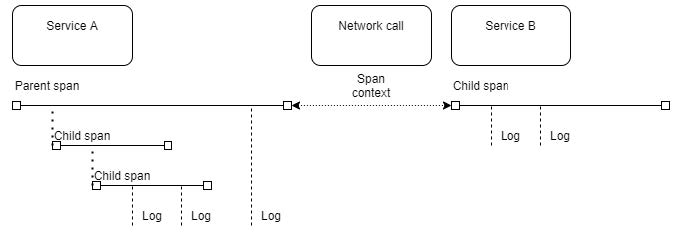
\includegraphics[width=0.9\textwidth]{content/4/chapter15/images/1.jpg}\\
Figure 15.1 – Single trace 
\end{center}

Two services communicate over a network. In Service A, we have one parent span that contains a child span and a single log. Child spans usually correspond to deeper function calls. A log represents the smallest piece of information. Each of them is timed and may contain additional information.

The network call to Service B preserves the span context. Even though Service B is executed in a different process on another machine, all of the information can be later reassembled as the transaction ID is preserved.

A piece of bonus information that we get from reassembling traces is the dependency graph between the services in our distributed system. As traces contain the entire call chain, it is possible to visualize this information and inspect unexpected dependencies.

\subsubsubsection{15.2.2\hspace{0.2cm}Choosing a tracing solution}

There are several possible solutions to choose from when implementing tracing. As you may imagine, there are both self-hosted and managed tools that you can use to instrument your applications. We will briefly describe the managed ones and focus on the self-hosted ones.

\hspace*{\fill} \\ %插入空行
\noindent
\textbf{Jaeger and OpenTracing}

One of the standards in distributed tracing is OpenTracing proposed by the authors of Jaeger. Jaeger is a tracer built for cloud-native applications. It addresses the problems of monitoring distributed transactions and propagating the tracing context. It's useful for the following purposes:

\begin{itemize}
\item 
Performance or latency optimization

\item 
Performing a root cause analysis

\item 
Analyzing the inter-service dependencies
\end{itemize}

OpenTracing is an open standard presenting an API that is independent of the tracer used. This means that when your application is instrumented using OpenTracing, you avoid lock-in to one particular vendor. If, at some point, you decide to switch from Jaeger to Zipkin, DataDog, or any other compatible tracer, you won't have to modify the entire instrumentation code.

There are many client libraries compatible with OpenTracing. You can also find many resources, including tutorials and articles that explain how to implement the API for your needs. OpenTracing officially supports the following languages:

\begin{itemize}
\item 
Go

\item 
JavaScript

\item 
Java

\item 
Python

\item 
Ruby

\item 
PHP

\item 
Objective-C

\item 
C++

\item 
C\#
\end{itemize}

There are also unofficial libraries available, and specific applications can export OpenTracing data as well. This includes Nginx and Envoy, both popular web proxies.

Jaeger also accepts samples in Zipkin format. We will cover Zipkin in the next section. What it means is that you don't have to rewrite the instrumentation from one format to another if you (or any of your dependencies) already use Zipkin. For all new applications, OpenTracing is the recommended approach.

Jaeger scales well. You can run it as a single binary or a single application container if you want to evaluate it. You may configure Jaeger for production use to use its own backend or a supported external one, such as Elasticsearch, Cassandra, or Kafka.

Jaeger is a CNCF graduated project. This means it has reached a similar level of maturity to Kubernetes, Prometheus, or Fluentd. Because of this, we expect it to gain even more support in other CNCF applications.

\hspace*{\fill} \\ %插入空行
\noindent
\textbf{Zipkin}

The main competitor for Jaeger is Zipkin. It's an older project, which also means it is more mature. Usually, more senior projects are also better supported, but in this case, the endorsement of CNCF plays in Jaeger's favor.

Zipkin uses its proprietary protocol to handle tracing. It has OpenTracing support available, but it may not be at the same maturity and support level as the native Jaeger protocol. As we've mentioned earlier, it is also possible to configure Jaeger to collect traces in Zipkin format. This means the two are, at least to some point, interchangeable.

The project is hosted under the Apache foundation, but is not considered a CNCF project. When developing cloud-native applications, Jaeger is a better alternative. If you are looking instead for an all-purpose tracing solution, it is worth considering Zipkin as well.

One drawback is that Zipkin doesn't have a supported C++ implementation. There are unofficial libraries, but they don't seem to be well-supported. Using a C++ OpenTracing library is the preferred way to instrument the C++ code.

\subsubsubsection{15.2.3\hspace{0.2cm}Instrumenting an application with OpenTracing}

This section will illustrate how to add instrumentation with Jaeger and OpenTracing to an existing application. We'll use the opentracing-cpp and jaeger-client-cpp libraries.

First, we want to set up the tracer:

\begin{lstlisting}[style=styleCXX]
#include <jaegertracing/Tracer.h>

void setUpTracer()
{
	// We want to read the sampling server configuration from the
	// environment variables
	auto config = jaegertracing::Config;
	config.fromEnv();
	// Jaeger provides us with ConsoleLogger and NullLogger
	auto tracer = jaegertracing::Tracer::make(
	"customer", config, jaegertracing::logging::consoleLogger());
	opentracing::Tracer::InitGlobal(
	std::static_pointer_cast<opentracing::Tracer>(tracer));
}
\end{lstlisting}

The two preferred methods for configuring a sampling server are either by using the environment variable, as we did, or by using a YAML configuration file. When using environment variables, we will have to set them up before running the application. The most important ones are as follows:

\begin{itemize}
\item 
JAEGER\_AGENT\_HOST: The hostname where the Jaeger agent is located

\item 
JAEGER\_AGENT\_POR: The port on which the Jaeger agent is listening

\item 
JAEGER\_SERVICE\_NAME: The name of our application
\end{itemize}

Next, we configure the tracer and supply the logging implementation. It is possible to implement a custom logging solution if the available ConsoleLogger is not enough. For container-based applications with a unified logging layer, the ConsoleLogger should be enough.

When we have the tracer set up, we want to add spans to the functions that we want to be instrumented. The following code does just that:

\begin{lstlisting}[style=styleCXX]
auto responder::respond(const http_request &request, status_code status,
const json::value &response) -> void {
	auto span = opentracing::Tracer::Global()->StartSpan("respond");
	// ...
}
\end{lstlisting}

This span may be used later to create child spans within a given function. It may also be propagated to deeper function calls as a parameter. This is how it appears:

\begin{lstlisting}[style=styleCXX]
auto responder::prepare_response(const std::string &name, const
std::unique_ptr<opentracing::Span>& parentSpan)
-> std::pair<status_code, json::value> {
	auto span = opentracing::Tracer::Global()->StartSpan(
	"prepare_response", { opentracing::ChildOf(&parentSpan->context())
	});
	return {status_codes::OK,
		json::value::string(string_t("Hello, ") + name + "!")};
}

auto responder::respond(const http_request &request, status_code status)
-> void {
	auto span = opentracing::Tracer::Global()->StartSpan("respond");
	// ...
	auto response = this->prepare_response("Dominic", span);
	// ...
}
\end{lstlisting}

Context propagation happens when we call the opentracing::ChildOf function. We may also pass the context over network calls using the inject() and extract() calls.













